\documentclass{beamer}

\usepackage[utf8]{inputenc}
\usepackage{graphicx}
\usepackage{booktabs}
\graphicspath{ {./Figures/} }

\title{Modeling Price and Popularity of AirBnB listings in New-York}
\author{Olivier Binette, Raphael Morsomme}
\institute{Department of Statistical Science, Duke University}
\date{02/20/2020}

\begin{document}

\frame{\titlepage}


\begin{frame} \frametitle{test}    
    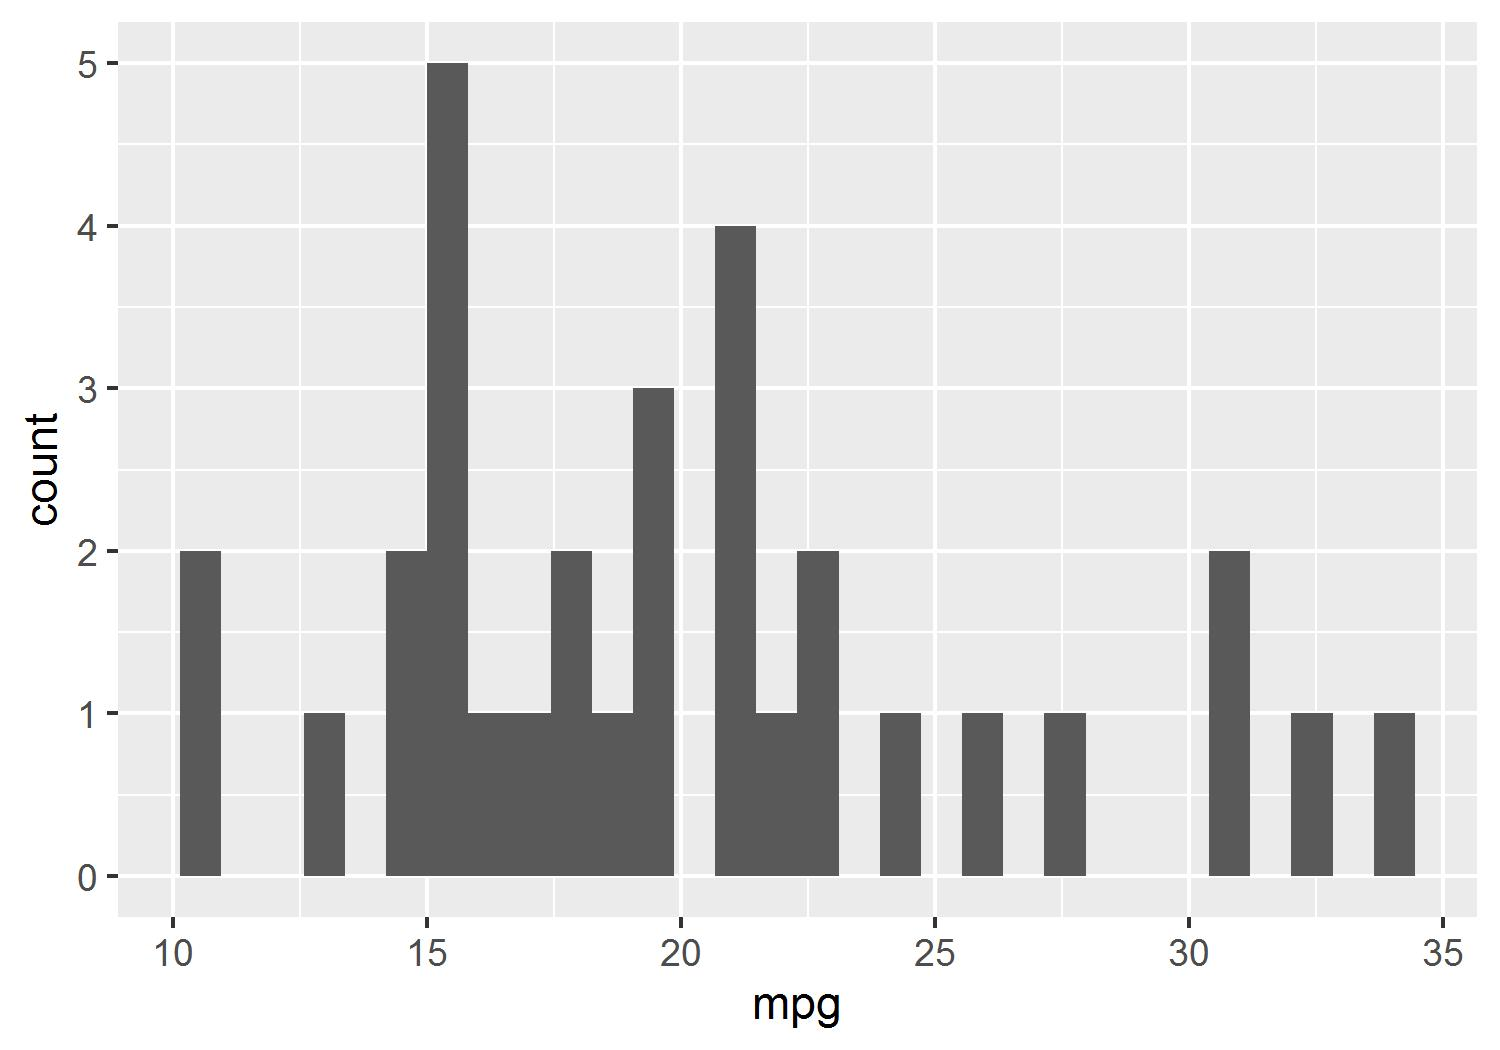
\includegraphics[scale = 0.8]{test.jpeg}
\end{frame}

\begin{frame} \frametitle{Conformal Predictors}

Prediction intervals that are
\begin{itemize}
	\item valid at a given significance level for \textit{finite} sample (Vovk, 2005)
	\item distribution-free
	\item universal
	\item individualized (Papadopoulos, 2009)
	\item only assume exchangeability
	\item cheap (Papadopoulos, 2002)
\end{itemize}
\end{frame}


\begin{frame} \frametitle{Inductive Conformal Prediction}

Given a labeled training set $\{z_i = (x_i, y_i)\}_{i=1}^n$ and an unlabeled test observation $x_{n+1}$,
\begin{enumerate}
	\item partition training set into a \textit{proper training} set $\{z_j\}_{j=1}^l$ and a \textit{calibration} set $\{z_k \}_{k=l+1}^n$
	\item fit predictive model on proper training set
	\item compute predictions $\hat{y}_k$ on calibration set and anomaly scores
	$$a(z_k) = |\hat{y}_k - y_k|, \quad k = l+1, \dots, n$$
	\item identify $a_\epsilon$, the $\epsilon^{\text{th}}$ percentile of the $\{a\}_{k=l+1}^n$
	\item compute prediction on test observation and set the prediction interval to be
	$$\{y: |\hat{y}_{n+1} - y| < a_\epsilon\}$$
	\end{enumerate}
\end{frame}


\begin{frame} \frametitle{Set up}
\begin{itemize}
	\item Test set is $10\%$ of data set
	\item Calibration set is $30\%$ of training set.
	\item repeat $100$ times to obtain the expected width of prediction intervals	
\end{itemize}
\end{frame}

\begin{frame} \frametitle{Results - Coverage}  
% latex table generated in R 3.5.2 by xtable 1.8-3 package
% Mon Feb 17 15:58:32 2020
\begin{table}[ht]
\centering
\begin{tabular}{rrlrr}
  \toprule
 & Significance & Set of Predictors & Mean Width & Coverage \\ 
  \midrule
1 & 0.500 & Extensive & 1.138 & 0.503 \\ 
  2 & 0.500 & Restricted & 1.370 & 0.501 \\ 
  3 & 0.750 & Extensive & 1.807 & 0.754 \\ 
  4 & 0.750 & Restricted & 2.109 & 0.749 \\ 
  5 & 0.900 & Extensive & 2.513 & 0.909 \\ 
  6 & 0.900 & Restricted & 2.801 & 0.897 \\ 
  7 & 0.950 & Extensive & 2.896 & 0.954 \\ 
  8 & 0.950 & Restricted & 3.212 & 0.951 \\ 
   \bottomrule
\end{tabular}
\caption{Coverage and Mean Width of Prediction Intervals} 
\end{table}

\end{frame}

\begin{frame} \frametitle{Results - Width}    
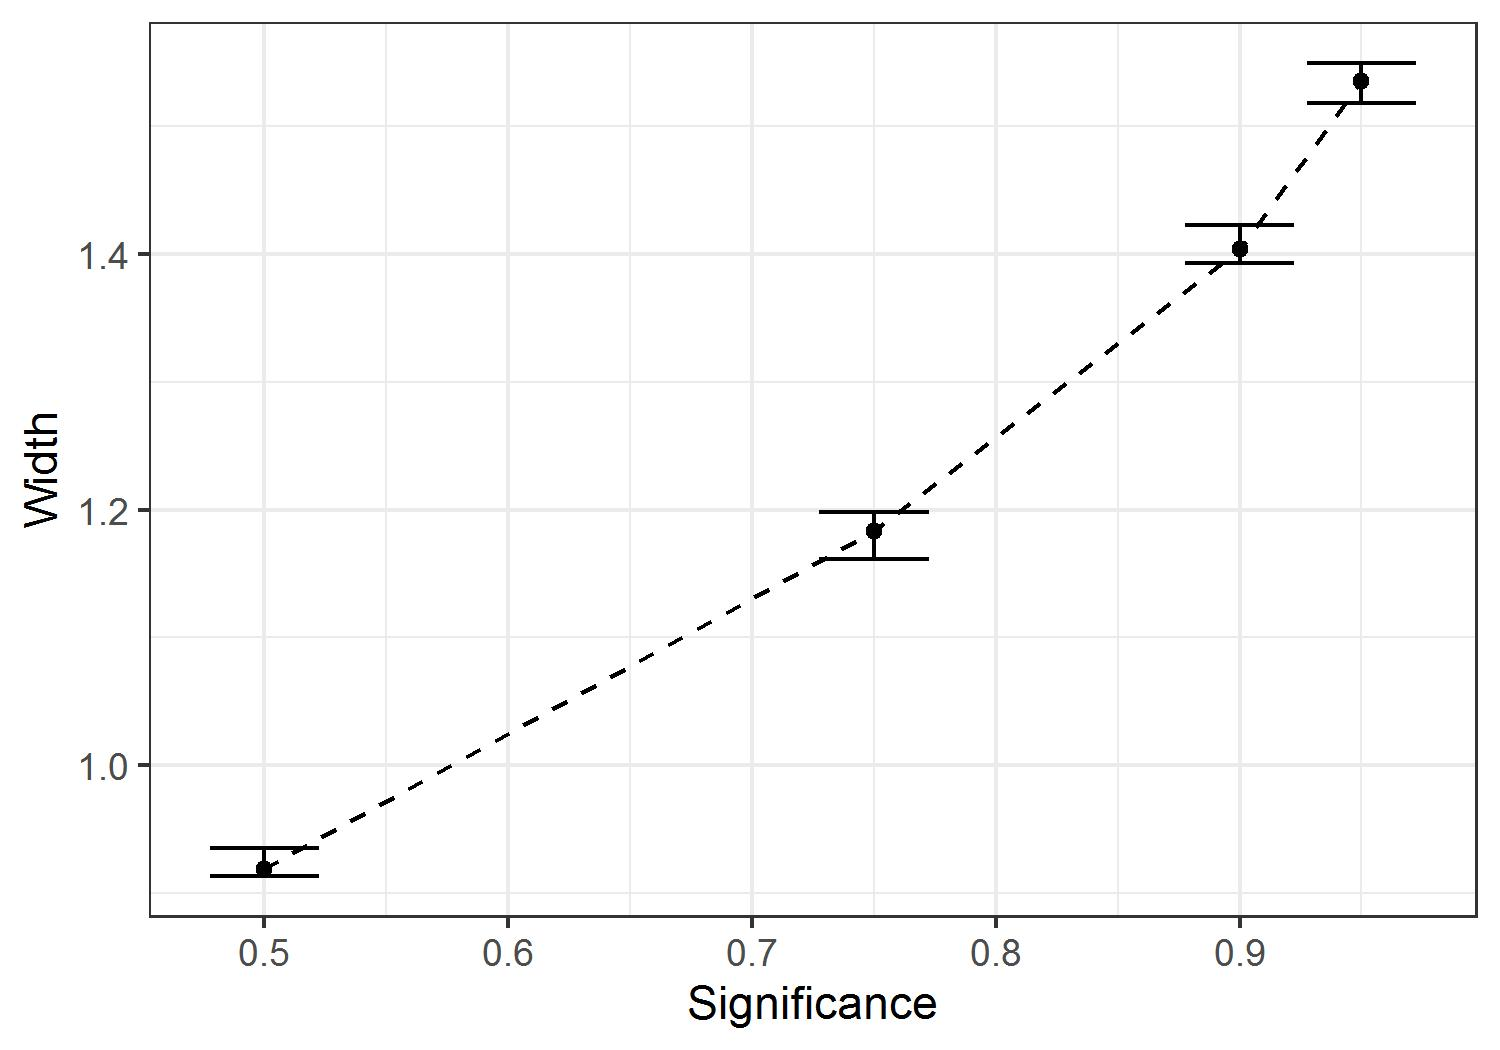
\includegraphics[scale = 0.8]{conformal.jpeg}
\end{frame}







\begin{frame}
\frametitle{References}
\footnotesize{
	\begin{thebibliography}{99} % Beamer does not support BibTeX so references must be inserted manually as below
		
		\bibitem[Vovk, 2005]{Whickam2009} Vovk, A. \\
		\newblock Tidy Data\\
		\newblock \emph{Journal}, month year
		
		\bibitem[Papadopoulos, 2002]{Valente2005} Valente, j. \\
		\newblock Apartment Rent Prediction Using Spatial Modeling\\
		\newblock \emph{Journal}, month year
		
		\bibitem[Papadopoulos, 2009]{Belasco2012} Belasco, E. \\
		\newblock Using a Finite Mixture Model of Heterogeneous Households to Delineate Housing Submarkets\\
		\newblock \emph{Journal}, month year
		
	\end{thebibliography}
}
\end{frame}
    






\end{document}
